\documentclass{standalone}
\usepackage{tikz}
\usepackage{amsmath}

\usetikzlibrary{arrows.meta,decorations.pathreplacing}

\tikzset{
    line/.style={
        thick
    },
    arrow/.style={
        line,
        ->,
        > = {
            Triangle[length=2.0mm, width=2.0mm]
        }
    }
}

% Switch to Sans Serif font.
\renewcommand{\familydefault}{\sfdefault}

\renewcommand{\wedge}{$\vphantom{\big|}$}


\begin{document}
\begin{tikzpicture}[xscale=1]
    \node (data) {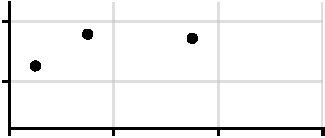
\includegraphics[width=4cm]{nps/translation_equivariance/data.pdf}};
    \node [right=2cm of data] (pred) {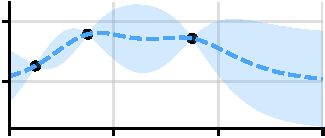
\includegraphics[width=4cm]{nps/translation_equivariance/pred.pdf}};
    \draw [arrow, ->] (data) -- node [above, midway] {$\phi$} (pred);
    \node [below=1cm of data] (datashifted) {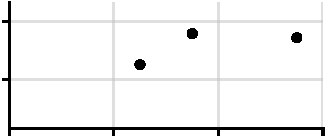
\includegraphics[width=4cm]{nps/translation_equivariance/data_shifted.pdf}};
    \draw [arrow, ->] (data) -- node [anchor=west] {shift} (datashifted);
    \node [right=2cm of datashifted] (predshifted) {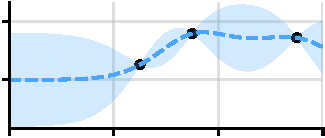
\includegraphics[width=4cm]{nps/translation_equivariance/pred_shifted.pdf}};
    \draw [arrow, ->] (datashifted) -- node [above, midway] {$\phi$} (predshifted);
    \draw [arrow, ->] (pred) -- node [anchor=west] {shift} (predshifted);
\end{tikzpicture}
\end{document}